\documentclass[11pt,a4paper]{article}

% The course limit is 3 pages, references included; check the page count
% after every edit (page 3 is full to the bottom).
\usepackage[utf8]{inputenc}
\usepackage[T1]{fontenc}
\usepackage{lmodern}
\usepackage{amsmath,amssymb}
\usepackage{graphicx}
\usepackage{booktabs}
\usepackage[margin=2cm]{geometry}
\usepackage{xcolor}
\usepackage[colorlinks=true,linkcolor=blue,citecolor=blue,urlcolor=blue]{hyperref}
\usepackage{enumitem}
\usepackage[numbers,sort&compress]{natbib}
\usepackage{titlesec}

\titlespacing*{\section}{0pt}{1.4ex plus .5ex}{0.7ex}
\titlespacing*{\subsection}{0pt}{1ex plus .3ex}{0.4ex}
\titlespacing*{\paragraph}{0pt}{0.6ex plus .2ex}{0.8em}
\usepackage[font=small,skip=3pt]{caption}
\setlength{\textfloatsep}{8pt plus 2pt}
\setlength{\floatsep}{6pt plus 2pt}
\setlist{nosep,leftmargin=*}
% Lets LaTeX stretch a line slightly instead of letting long bold names stick out.
\setlength{\emergencystretch}{2em}

\newcommand{\sam}{SAM~2}
\newcommand{\gdsam}{Grounded-SAM~2}

\begin{document}

\begin{center}
    {\Large\bfseries Breaking SAM 2: An Evaluative Benchmark on Extreme Object Evolution}\\[0.6em]
    Yarin Ben Shitrit, Benjamin A. Cohen, Eliezer Mashihov, Ido Avital\\
    {\small Modern Computer Vision 00970202 final project}\\
    {\small Faculty of Data and Decision Sciences, Technion -- Israel Institute of Technology}\\
\end{center}
\suppressfloats[t] % keep Fig.~1 from floating above the title

\begin{abstract}
\noindent
Standard video segmentation benchmarks mostly contain objects with a stable
shape and appearance. We present a small, inference-only stress test that measures
\emph{when}, \emph{how}, and \emph{under which transformation} \sam{} fails,
on 52 clips from M3-VOS, VOST, DAVIS~2017, and VOT: 14 with topology/state
change, 14 with extreme scale or viewpoint change, 10 with illumination
change, and 14 controls. We compare \sam{} prompted with a verified box to
\gdsam{}, where Grounding DINO gives the first box from a text prompt, and
report detector misses separately from propagation failures. With a verified
box, \sam{} fails on 12 of 14 topology clips (median 2.0\,s after the event)
and 5 of 10 illumination clips, but on only 1 of 14 scale clips and no
control clip. Grounding DINO fails to initialize on 11 of 52 clips; on the
other 41, \gdsam{} is only 2.0 $J\&F$ points below \sam{}. Code:
\url{https://github.com/YarinBS/breaking-sam2}.
\end{abstract}

% =========================================================
\section{Introduction}
% =========================================================
\sam{}~\cite{ravi2024sam2} extends the promptable Segment Anything
Model~\cite{kirillov2023sam} to video: the object is prompted once, and a
streaming memory of the prompted frame and of recent predictions is used to
segment every new frame. In \gdsam{}~\cite{ren2024grounded}, a box from the
open-set detector Grounding DINO~\cite{liu2023groundingdino} for a free-text
phrase replaces the manual prompt. Uses such as dataset labeling and robot
manipulation often contain objects that do not behave like the rigid objects
of standard benchmarks: vegetables are cut, water is poured, a car grows from a few pixels
to half of the frame, the lighting changes within one frame. \sam{}'s memory
assumes that the target keeps similar visual cues over time, and amorphous
targets such as ``water'' are hard to describe with one box. We ask \emph{when, how, and under which
transformation} \sam{} fails, keep the two error sources of \gdsam{} (a wrong
first box, later drift) apart, and study:
(i)~which disruption causes the earliest and most severe degradation;
(ii)~whether failures are abrupt, gradual, or recoverable;
(iii)~how sensitive propagation is to the initial prompt;
and (iv)~whether text-guided initialization helps or only adds a
first-frame detection failure.

\paragraph{Related work.}
DAVIS~\cite{perazzi2016benchmark,pont2017davis} and
YouTube-VOS~\cite{xu2018youtube} defined the standard region ($J$) and
boundary ($F$) metrics but mostly contain objects with a stable identity;
VOST~\cite{tokmakov2023vost} and M3-VOS~\cite{chen2025m3vos} target objects
that change state or phase. We test a promptable \emph{foundation} model and
its text-initialized variant, add scale/viewpoint and illumination changes,
and report \emph{temporal} failure behavior, not only mean accuracy.

% =========================================================
\section{Method}
% =========================================================
\begin{figure}[t]
    \centering
    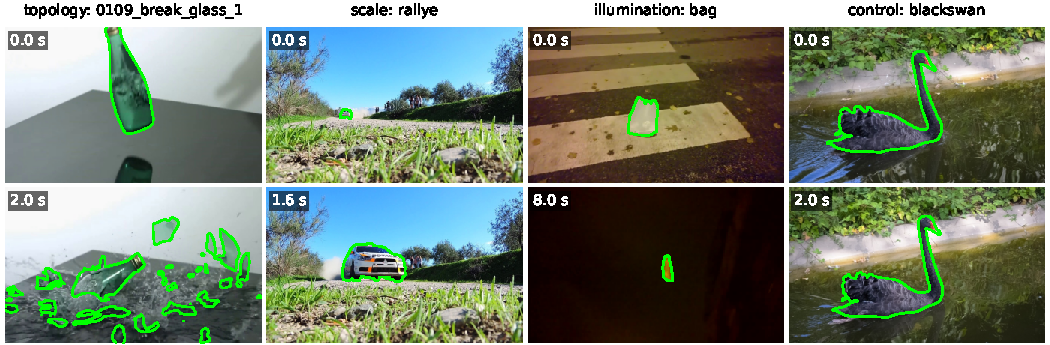
\includegraphics[width=\textwidth]{figures/examples.pdf}
    \caption{One clip per category, ground truth in green. Top: frame~0
    (prompted). Bottom: a later frame after the event.}
    \label{fig:examples}
\end{figure}

\paragraph{Benchmark.}
Each category breaks a different assumption of \sam{}'s memory: that the
object keeps its form, its size, or its appearance (Fig.~\ref{fig:examples}).
\textbf{Topology/state} (14 clips; M3-VOS 8, VOST validation 6): the object is
cut, broken, or torn, it flows, melts, or it is smoke.
\textbf{Scale/viewpoint} (14): the object's size changes by at least $5\times$
(up to $170\times$), or the view rotates strongly. \textbf{Illumination} (10):
mostly abrupt light changes (muzzle flashes, stage lights, darkness), three
gradual. \textbf{Control} (14): ordinary motion, nearly constant size and
lighting, one object of the target's class. Scale, illumination, and control
clips come from DAVIS~2017 (11, 3, 11) and VOT-ST2022~\cite{kristan2022vot}
(3, 7, 3). All clips (1.5--35\,s) have expert per-frame ground truth and were
fixed before any model was run on them. Each
clip has a fixed text prompt and an event frame $t_{\mathrm{ev}}$, checked by
eye: the first lasting split or area change (topology), the first $5\times$
area change (scale), or the start of the light change (illumination).

\paragraph{Pipelines.}
Both conditions use \sam{}.1 Hiera-B+ and propagate from frame~0 to the end.
(A)~\textbf{\sam{}}: a manually verified box (tight around the frame-0
ground truth) isolates propagation errors. (B)~\textbf{\gdsam{}}: the top box of Grounding DINO (tiny; box/text
thresholds 0.35/0.25) on frame~0 prompts \sam{}; without a detection the
masks are empty. This, and any run with $J_0<0.5$, is an
\emph{initialization failure}, not a propagation failure.
(C)~\textbf{Prompt sensitivity}: (A) with the box shifted right and down by
10\% of its size, and enlarged by 20\% around its center.

\paragraph{Metrics.}
For each annotated frame $t$ with prediction $P_t$ and ground truth $G_t$:
$J_t=|P_t\cap G_t|/|P_t\cup G_t|$, the boundary F-measure $F_t$ (tolerance
0.8\% of the image diagonal), and $J\&F=(J+F)/2$; to explain \emph{how} a clip
fails also the signed area error, the number of connected components of
$P_t$, and the temporal IoU between $P_{t-1}$ and $P_t$. The pre-registered
first failure is
\begin{equation}
    t_{\mathrm{fail}}=\min\{\,t_i : J_{t_i}<0.5 \;\wedge\; J_{t_{i+1}}<0.5\,\},
    \qquad \Delta=(t_{\mathrm{fail}}-t_{\mathrm{ev}})/\mathrm{fps}.
\end{equation}
Clips without such a run are \emph{censored}; controls use $t_{\mathrm{ev}}=0$.
Recovery is a later run of two frames with $J\ge0.5$. A failure is
\emph{abrupt} when the temporal IoU at $t_{\mathrm{fail}}$ is below 0.5 and
\emph{gradual} otherwise.

% =========================================================
\section{Results}
% =========================================================
All runs use one NVIDIA A100 GPU, PyTorch 2.14, \sam{} (commit
\texttt{2b90b9f}), and Transformers 4.50; \texttt{python
reproduce\_results.py} downloads the data, runs all conditions, and prints
every number below. On another GPU (an NVIDIA H200) the means changed by at
most 0.2 $J\&F$ points; all failure counts and median $\Delta$ values stayed
the same.



\begin{figure}[t]
    \centering
    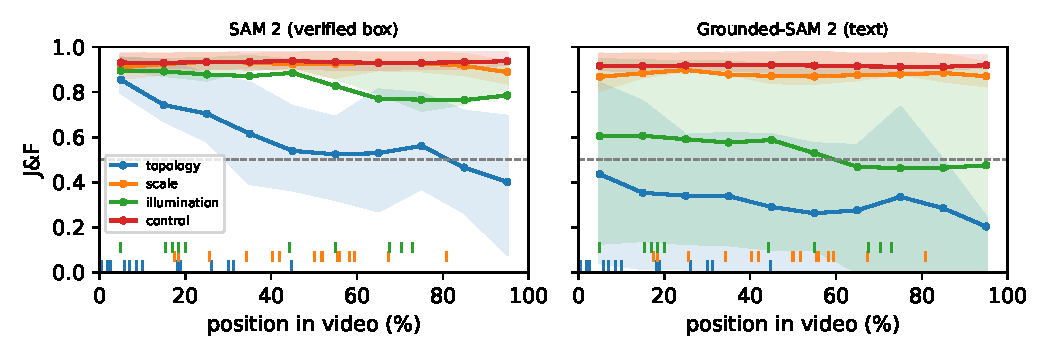
\includegraphics[width=0.92\textwidth]{figures/jf_progress.pdf}
    \caption{Mean $J\&F$ (band: IQR over clips) against the position in the
    clip (0\% = prompted frame); ticks mark each clip's event. Left: \sam{}.
    Right: \gdsam{}, including initialization failures ($J\&F=0$).}
    \label{fig:progress}
\end{figure}

\begin{figure}[t]
\begin{minipage}[b]{0.6\textwidth}
\centering
\footnotesize
\setlength{\tabcolsep}{3.5pt}
\begin{tabular}{lc ccc cccc}
\toprule
& & \multicolumn{3}{c}{\sam{} (box)} & \multicolumn{4}{c}{\gdsam{} (text)} \\
\cmidrule(lr){3-5}\cmidrule(lr){6-9}
Category & Clips & $J\&F$ & Fail & $\tilde\Delta$ & $J\&F$ & Fail & $\tilde\Delta$ & Init \\
\midrule
Topology     & 14 & 59.5 & 86\% & 2.0 & 31.2 & 86\% & 1.9 & 50\% \\
Scale        & 14 & 92.1 & 7\%  & 9.5 & 87.8 & 7\%  & $-4.0$ & 0\%  \\
Illumination & 10 & 83.3 & 50\% & 1.1 & 53.8 & 33\% & 0.8 & 40\% \\
Control      & 14 & 93.3 & 0\%  & --  & 91.7 & 0\%  & --  & 0\%  \\
\midrule
All          & 52 & 82.0 & 35\% & 2.0 & 67.1 & 22\% & 1.1 & 21\% \\
\bottomrule
\end{tabular}
\captionof{table}{Fail: share of clips with a first failure; $\tilde\Delta$:
median time from event to failure (s); Init: \gdsam{} initialization
failures. \gdsam{} Fail and $\tilde\Delta$ use initialized clips only.}
\label{tab:results}
\end{minipage}\hfill
\begin{minipage}[b]{0.37\textwidth}
\centering
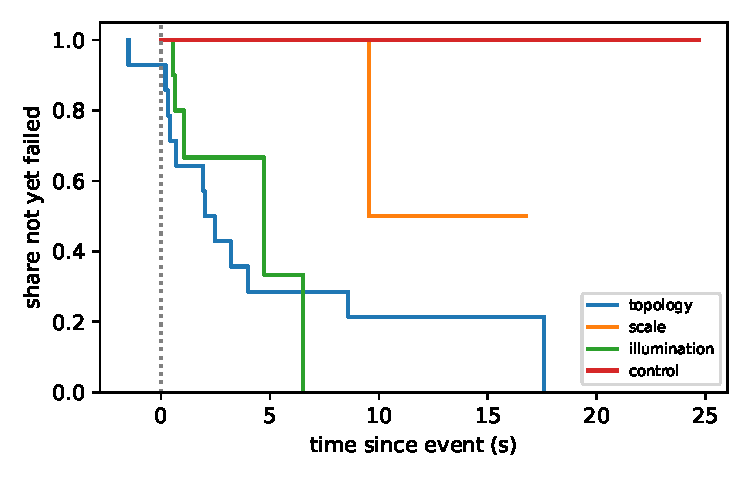
\includegraphics[width=\textwidth]{figures/survival.pdf}
\caption{Kaplan--Meier survival until the first failure of \sam{} (verified
box), from the event.}
\label{fig:temporal}
\end{minipage}
\end{figure}

\paragraph{Degradation across the video.}
With the verified box, all categories start at a similar level (mean $J\&F$
0.85--0.93 in the first 10\% of the clip; Fig.~\ref{fig:progress}), so the
later differences come from propagation. Topology clips degrade steadily after
their early events (median at 9\% of the clip) to 0.40 at the end;
illumination clips drop after their events (median at 32\%) from 0.89 to
0.79; scale and control clips stay at about 0.9. With \gdsam{}, topology and
illumination start much lower (0.44 and 0.61), and the gap to \sam{} does not
grow later.

\paragraph{Which disruption breaks \sam{} first? (RQ i)}
Topology/state change causes the earliest and most frequent failures: 12 of
14 clips fail, with a median $\Delta$ of 2.0\,s (Table~\ref{tab:results},
Fig.~\ref{fig:temporal}). Illumination change is second: 5 of 10 clips fail
(median 1.1\,s), e.g.\ \texttt{bag} after it enters near darkness and
\texttt{shooting} after the muzzle flashes, while gradual light changes cause
no failure. No control clip fails. Surprisingly, only 1 of 14 scale clips
fails (\texttt{helicopter}, 9.5\,s after the event, at 0.05\% of the image);
objects that grow up to $170\times$ are tracked without failure.

\paragraph{Abrupt, gradual, or recoverable? (RQ ii)}
Of the 18 \sam{} failures, 9 are abrupt and 9 gradual (topology: 5 of 12
abrupt). 13 of 18 failed clips later have two consecutive frames with
$J\ge0.5$ again, but this is not good tracking: the mean worst-frame $J$ of
topology clips is 0.20 (0.86 for controls), and their masks have twice as
many connected components (2.7 vs.\ 1.3).

\paragraph{Prompt sensitivity (RQ iii).}
Shifting the verified box by 10\% of its size lowers the mean $J\&F$ by 5.5
points and makes failures 1.4\,s earlier (on clips that fail in both runs);
enlarging it by 20\% costs 6.6 points and 1.1\,s. Each change flips the
failure status of 3 of 52 clips.

\paragraph{Initialization vs.\ propagation (RQ iv).}
Grounding DINO fails to initialize on 11 of 52 clips: 7 of 14 topology and 4
of 10 illumination clips, but no scale or control clip. The prompts name
amorphous or small targets, and scenes often contain several objects of the
same class: on \texttt{0018\_cut\_pepper\_5} the top box (score 0.70) covers
the whole bunch of peppers, while the second box (0.41) would have fit the
target. On the 41 correctly initialized clips, \gdsam{} is 2.0 $J\&F$ points
below \sam{}, almost all from three clips with a looser detector box
(\texttt{helicopter}, \texttt{soapbox}, \texttt{hike}). Text initialization
therefore mainly adds a first-frame failure mode.

% =========================================================
\section{Discussion}
% =========================================================
\sam{} is robust to large changes of scale and viewpoint and to gradual
lighting changes, but it breaks when the object itself changes (failures in
86\% of topology clips, about 2\,s after the event) and, in half of the
illumination clips, under abrupt light changes. When $J$
falls while the temporal IoU stays high, the mask is stable but wrong: the
memory keeps the old appearance while the object changes; when both drop, the
target is lost suddenly. For
practical systems this suggests re-prompting or refreshing the memory after a
large change of the object, and checking the first-frame detection before
trusting a text-initialized track.

\paragraph{Limitations.}
The benchmark is small, and clip selection may add bias. VOST is sampled at
5\,fps; clip lengths differ between datasets; event times are estimated
from the ground truth; several VOT clips combine a light change with scale
change. An overlap of \sam{}.1's undocumented training data with DAVIS cannot
be excluded. All results are for one checkpoint per model.

% ---------------------------------------------------------
\footnotesize
\setlength{\bibsep}{0pt}
\begin{thebibliography}{10}

\bibitem{ravi2024sam2}
N.~Ravi et~al. SAM 2: Segment anything in images and videos. \emph{arXiv:2408.00714}, 2024.

\bibitem{kirillov2023sam}
A.~Kirillov et~al. Segment anything. In \emph{ICCV}, 2023.

\bibitem{liu2023groundingdino}
S.~Liu et~al. Grounding DINO: Marrying DINO with grounded pre-training for open-set object detection. In \emph{ECCV}, 2024.

\bibitem{ren2024grounded}
T.~Ren et~al. Grounded SAM: Assembling open-world models for diverse visual tasks. \emph{arXiv:2401.14159}, 2024.

\bibitem{perazzi2016benchmark}
F.~Perazzi et~al. A benchmark dataset and evaluation methodology for video object segmentation. In \emph{CVPR}, 2016.

\bibitem{pont2017davis}
J.~Pont-Tuset et~al. The 2017 DAVIS challenge on video object segmentation. \emph{arXiv:1704.00675}, 2017.

\bibitem{xu2018youtube}
N.~Xu et~al. YouTube-VOS: A large-scale video object segmentation benchmark. In \emph{ECCV}, 2018.

\bibitem{chen2025m3vos}
Z.~Chen et~al. M3-VOS: Multi-phase, multi-transition, and multi-scenery video object segmentation. In \emph{CVPR}, 2025.

\bibitem{kristan2022vot}
M.~Kristan et~al. The tenth visual object tracking VOT2022 challenge results. In \emph{ECCV Workshops}, 2022.

\bibitem{tokmakov2023vost}
P.~Tokmakov, J.~Li, and A.~Gaidon. Breaking the ``object'' in video object segmentation. In \emph{CVPR}, 2023.

\end{thebibliography}

\end{document}
